\documentclass[a4paper,16pt]{article}
\usepackage[a4paper, total={6in, 8in}]{geometry}

\usepackage{euscript}
\usepackage[utf8]{inputenc}
\usepackage[english,ukrainian]{babel}
\usepackage{mathtext}
\usepackage{epigraph}
\usepackage{indentfirst}
\usepackage{graphicx}
\usepackage{amsmath, amsthm,amsfonts,amsmath,amssymb,amscd}
\usepackage{mathrsfs}
\usepackage{apacite}
\usepackage{tabularx}
\usepackage{tikz}
\usepackage{hyperref}

\usepackage{longtable,booktabs}

\graphicspath{{images/}}
\DeclareGraphicsExtensions{.png,.jpg}

% ************************************************************* %
%  Визначення математичних оточень та роботи з формулами
% ************************************************************* %

\theoremstyle{plain}
\newtheorem{theorem}{\indent Теорема}[chapter]
\newtheorem{claim}{\indent Твердження}[chapter]
\newtheorem{lemma}{\indent Лема}[chapter]	
\newtheorem{corollary}{\indent Наслідок}[chapter]

\theoremstyle{definition}
\newtheorem{definition}{\indent Означення}[chapter]
\newtheorem{algorithm}{\indent Алгоритм}[chapter]
\newtheorem{problem}{\indent Задача}[chapter]
\newtheorem{example}{\indent Приклад}[chapter]
\theoremstyle{remark}
\newtheorem*{remark}{\indent\textbf{Зауваження}}
\renewenvironment{proof}{{\indent\bfseries Доведення.~}}{\qed}

% змінюємо формат нумерації формул
\renewcommand{\theequation}{\arabic{chapter}.\arabic{equation}}

% команди для заборони розриву формул у небажаному місці
\binoppenalty=10000
\relpenalty=10000


% ************************************************************* %
%  Ненумеровані розділи
% ************************************************************* %

% команда для створення ненумерованого розділу, який тим не менше показується в змісті
\newcommand{\uchapter}[1]{\chapter*{#1}\addcontentsline{toc}{chapter}{#1}} 

\newcommand{\intro}{\uchapter{Вступ}}                   % для створення вступу використаємо команду \uchapter
\newcommand{\conclusions}{\uchapter{Висновки}}          % для створення висновків використаємо команду \uchapter
\newcommand{\shortings}{\uchapter{Перелік умовних позначень, скорочень і термінів}}
                                                        % для створення переліку умовних позначень використаємо команду \shortings

\newcommand{\chapconclude}[1]{\section*{Висновки до розділу #1} \addcontentsline{toc}{section}{Висновки до розділу #1}}

\def\checkmark{\tikz\fill[scale=0.4](0,.35) -- (.25,0) -- (1,.7) -- (.25,.15) -- cycle;} 

%основний документ
\begin{document}


% Титульный лист
	\thispagestyle{empty}
	
	\begin{center}
		НАЦІОНАЛЬНИЙ ТЕХНІЧНИЙ УНІВЕРСИТЕТ УКРАЇНИ \par
		<<КИЇВСЬКИЙ ПОЛІТЕХНІЧНИЙ ІНСТИТУТ ім. Ігоря СІКОРСЬКОГО>>\par
		НАВЧАЛЬНО-НАКУОВИЙ ФІЗИКО-ТЕХНІЧНИЙ ІНСТИТУТ\par
		
		\vspace{60mm}
		{\huge Звіт за темою:\par
			\LARGE <<Криптоаналiз асиметричних криптосистем на прикладi атак на криптосистему RSA>>\par}
		
	\end{center}
	
	\vspace{50mm}
	\begin{flushright}
		Виконав студент
		
		групи ФІ-32мн
		
		Кріпака Ілля
		
	\end{flushright}
	
	\vspace{27mm}
	\begin{center}
		{Київ~--- 2024}
	\end{center}
	
\newpage

\pagenumbering{gobble}
\cleardoublepage
\pagenumbering{arabic}

\setcounter{page}{2} 

\section{Мета практикуму}

Ознайомлення з пiдходами побудови атак на асиметричнi криптосистеми на прикладi атак на криптосистему RSA, а саме атаки на основi китайської теореми про лишки, що є успiшною при використаннi однакового малого  значення вiдкритої експоненти для багатьох користувачiв, та атаки <<зустрiч посерединi>>, яка можлива у випадку, якщо шифротекст є невеликим числом, що є добутком двох чисел.

Практично ознайомитися із принципами статистичних методiв розрiзнення змiстовного тексту вiд випадкової послiдовностi, порівняти їх.

\subsection{Постановка задачі та варіант}
У даній роботі виконував варіант №4 як і звичайний так і простий.


\begin{tabularx}{\textwidth}{X|X}
	\textbf{Треба виконати} & \textbf{Зроблено} \\
	Провести атаки та навести результати включно із часом їх виконання & \checkmark \\
\end{tabularx}


\section{Хід роботи/Опис труднощів}
    У ході роботи над даною лабораторною роботою було дуже просто реалізовано атаку малої експоненти, так як код для вирішення ситеми рівнянь уже був готовий і реалізований у попередніх лабах із асиметричної криптографії. Якщо говорити щодо атаки <<зустріч посередині>>, то чомусь думав, що код не працює, а це лише довго обчислювалося піднесення до степеня. Якщо не враховувати свої власні непопрозуміння, то проблем особливих не було.

\section{Результати дослідження}
У ході роботи було успішно на практиці проведено атаку на основі Китайської теореми про лишки та атаку <<зустріч посередині>>.

\section{Результат проведення атаки на основі Китайської теореми про лишки}
Атака була проведено успішно, адже значення ШТ та $m^e$ співпали.

        \begin{figure}[!h]
            \centering
            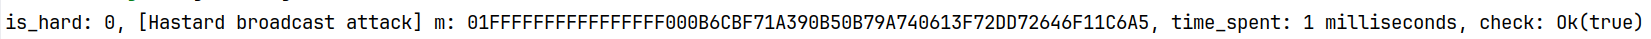
\includegraphics[width=0.5\linewidth]{Images/chinese_easy.png}
            \caption{Атака на легкий варіант.}
            \label{fig:chinese_easy}
        \end{figure}

        \begin{figure}[!h]
            \centering
            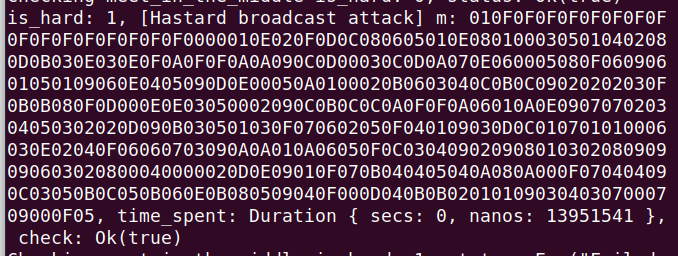
\includegraphics[width=0.5\linewidth]{Images/chinese_hard.png}
            \caption{Атака на звичайний варіант.}
            \label{fig:chinese_hard}
        \end{figure}

В результаті проведедння атаки отримав такі часові результати:
\begin{itemize}
    \item для легкого варіанту \textbf{time.spent} $=0.001804$ секунди;  
    \item для звичайного варіанту \textbf{time.spent} $=0.0514$ секунди.
\end{itemize}

\section{Результат проведення атаки <<зустріч посередині>>}
Атака була проведено успішно, адже значення ШТ та $m^e$ співпали.

\begin{figure}[!h]
            \centering
            
\includegraphics[scale=0.35]{Images/middle_easy.png}
            \caption{Атака на легкий варіант разом із повідомленням m та перевіркою на правильність.}
            \label{fig:middle_easy}
        \end{figure}

В результаті проведедння атаки отримав такі часові результати:
\begin{itemize}
    \item для легкого варіанту \textbf{time.spent} $=9$ хвилин;  
    \item для звичайного варіанту \textbf{time.spent} $=?$ не зміг дочекатися.
\end{itemize}

\subsection{Маленьке порівняння швидкодії із повним перебором}
На жаль, не проводилося, так як бачу скільки програма виконувала звичайний варіант по часу, не думаю, що саме моя програма виконає перебір швидше, буде тільки довше.

\section{Висновки}
В даному практикумі за допомогою програмної реалізації на практиці ознайомилися із пiдходами побудови атак на асиметричнi криптосистеми на прикладi атак на криптосистему RSA, а саме атаки на основi китайської теореми про лишки та атаки <<зустрiч посерединi>>. Перша атака вийшла добре, але друга за допомоги неоптимізованої реалізації працює дуже довго. Щоб покащити алгортими досить будде використати інший крейт із ефективнішою операцією піднесення до степеня.
% \begin{figure}
%     \centering
%     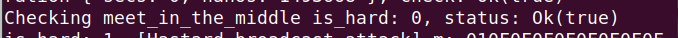
\includegraphics[width=0.5\linewidth]{middle_easy_check.png}
%     \caption{Enter Caption}
%     \label{fig:enter-label}
% \end{figure}


\end{document}

